\documentclass[tcc,capa]{texufpel}

\usepackage[utf8]{inputenc} % acentuacao
\usepackage{graphicx} % para inserir figuras
\usepackage[T1]{fontenc}

\hypersetup{
    hidelinks, % Remove coloração e caixas
    unicode=true,   %Permite acentuação no bookmark
    linktoc=all %Habilita link no nome e página do sumário
}

\unidade{Centro de Desenvolvimento Tecnológico}
\curso{Engenharia de Computação}
\nomecurso{Bacharelado em Engenharia de Computação}
\titulocurso{Bacharel em Engenharia de Computação}

\title{Proposta de exploração da plataforma Ethereum como base a aplicações em Fog Computing}

\author{Santos}{Gustavo Fernandes dos}
\advisor[Prof.~Dra.]{Reiser}{Renata Hax Sander}
\coadvisor[Prof.~Dr.]{Pilla}{Maurício}
%\collaborator[Prof.~Dr.]{Aguiar}{Marilton Sanchotene de}

%Palavras-chave em PT_BR
\keyword{ethereum}
\keyword{blockchain}
\keyword{internet das coisas}
\keyword{computação na borda}

%Palavras-chave em EN_US
\keywordeng{ethereum}
\keywordeng{blockchain}
\keywordeng{internet-of-things}
\keywordeng{edge computing}

\begin{document}

\renewcommand{\advisorname}{Orientadora}           %descomente caso tenhas orientadora
%\renewcommand{\coadvisorname}{Coorientadora}      %descomente caso tenhas coorientadora

\newcommand{\bchain}{\textit{blockchain} }
\newcommand{\Bchain}{\textit{Blockchain} }

\maketitle 

\sloppy

\fichacatalografica

\folhadeaprovacao

%Opcional
\begin{dedicatoria}
  Dedico\ldots bla blabla blablabla bla. Bla blabla blablabla bla.\\
  Bla blabla blablabla bla. Bla blabla blablabla bla.
\end{dedicatoria}

%Opcional
\begin{agradecimentos}
  Bla blabla blablabla bla.  Bla blabla blablabla bla.  Bla blabla blablabla
  bla.  Bla blabla blablabla bla.  Bla blabla blablabla bla.  Bla blabla
  blablabla bla.  Bla blabla blablabla bla.  Bla blabla blablabla bla.  Bla
  blabla blablabla bla.  Bla blabla blablabla bla.  Bla blabla blablabla bla.
  Bla blabla blablabla bla.  Bla blabla blablabla bla.  Bla blabla blablabla
  bla.  Bla blabla blablabla bla.  Bla blabla blablabla bla.  Bla blabla
  blablabla bla.  Bla blabla blablabla bla.  Bla blabla blablabla bla.  Bla
  blabla blablabla bla.  Bla blabla blablabla bla.
\end{agradecimentos}

%Opcional
\begin{epigrafe}
  Bla blabla blablabla bla.\\
  Bla blabla blablabla bla.\\
  Bla blabla blablabla bla.\\
  Bla blabla blablabla bla.\\
  Bla blabla blablabla bla.\\
  {\sc --- Fulano de Tal}
\end{epigrafe}

%Resumo em Portugues (no maximo 500 palavras)
\begin{abstract}
  resumo
\end{abstract}

\begin{englishabstract}%
  {Titulo do Trabalho em Inglês}
  
	abstract
\end{englishabstract}

%Lista de Figuras
\listoffigures

%Lista de Tabelas
\listoftables

%lista de abreviaturas e siglas
\begin{listofabbrv}{SPMD}
        \item[DAG] Directed Acyclic Graph
        \item[DHT] Distributed Hash Table
        \item[DLT] Distributed Ledger Technology
        \item[EUA] External User Account 
        \item[IOT] Internet of Things
        \item[IPFS] Interplanetary File System
        \item[KEC] Keccak-256
        \item[KEC512] Keccak-512
        \item[MPT] Merkle Patricia Tree
        \item[PoS] Proof of Stake
        \item[PoW] Proof of Work
\end{listofabbrv}

%Sumario
\tableofcontents

\chapter{Introdução}

    Um marco para a economia foi o desenvolvimento de formas de monetização digital. O primeiro indício da "era das moedas digitais" foi através de David Chaum, que propôs a ideia de dinheiro virtual em 1983 \cite{chaum1983blind}. A ideia de Chaum era a criação de uma moeda criptográfica capaz de servir para pagamentos ao mesmo tempo em que as partes envolvidas são anônimas, para isto, Chaum elegeu três propriedades fundamentais para que sua moeda virtual seja viável: 
	
	\begin{itemize}
	    \item Inabilidade de terceiros rastrear quem, quando e a quantidade de valor transferido entre os envolvidos;
	    \item Habilidade de participantes provarem que realizaram uma movimentação de valores em determinadas circunstâncias;
	    \item Habilidade de parar a movimentação de valores em caso de fraude.
	\end{itemize}
	
	Esta idealização rudimentar de dinheiro virtual era capaz de prover anonimidade entre os envolvidos, mas foi desastroso por centralizar as operações.
	
	A primeira manifestação de uma moeda virtual que realizava prova de trabalho para comprovar a autenticidade de transações entre usuários foi o \textit{B-Cash} definido por Wei Dai, entretanto o seu trabalho não é claro sobre o mecanismo por trás da prova de trabalho \cite{buterin2014next}. Adam Back propôs mais tarde o \textit{HashCash} que usava o método de resolução de enigmas para dar suporte ao valor monetário da moeda \cite{back2002hashcash}, entretanto a definição do \textit{HashCash} peca na veracidade sobre o que é definido e o que é de fato implementado.
	
	O Bitcoin é o primeiro e maior caso de sucesso em moedas digitais. O sistema proposto por \cite{nakamoto2008bitcoin} busca uma forma de realizar transações financeiras entre duas partes cuja autenticidade possa ser provada sem o intermédio de um terceiro agente. As transações no Bitcoin são computacionalmente impossíveis de serem revertidas uma vez que são aceitas, mineradas e adicionadas no livro público de transações.
	
	O livro público de transações é uma estrutura de dados organizada em blocos e distribuída em vários nós que compõe a rede do Bitcoin. Tal organização é uma cadeia de blocos ligados, popularmente \bchain. A inovação no Bitcoin reside no uso de \bchain em um sistema que garante transações não fraudulentas, disponibilidade contínua e a não necessidade de terceiros na movimentação de fundos. Um dos mecanismos que o Bitcoin utiliza é uma prova matemática que uma quantidade significante de trabalho sobre cada transação foi realizada e que esta transação é válida. 
	
	A prova de que uma transação não é falsa vem da organização das transações. Cada bloco que compõe a \bchain contém, não exclusivamente, um conjunto de transações e uma prova de trabalho, que é um número especial cuja hash do bloco começa com uma quantidade específica de zeros. A quantidade de zeros no início da hash do bloco indica a dificuldade para provar que o bloco é válido, quanto maior a dificuldade da prova, mais zeros existirão no início da hash do bloco e maior será o tempo para descobrir o número especial.
	
	A garantia da ordem dos blocos ocorre ao armazenar em cada novo bloco, a hash que descreve o bloco anterior. Este mecanismo garante que qualquer mudança no bloco anterior é reconhecida e acaba invalidando a ramificação no qual o novo bloco foi adicionado. A Figura \ref{fig:blockchain-basica} ilustra este mecanismo.
	
	\begin{figure}[h!]
        \centering
        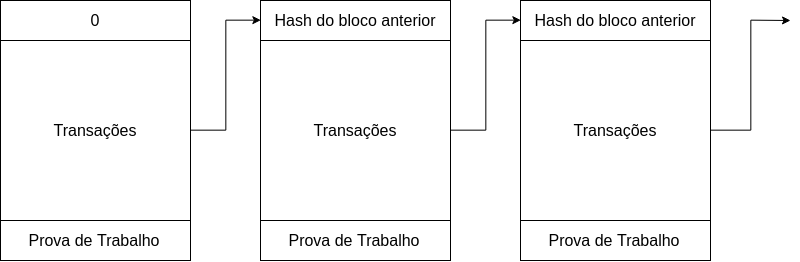
\includegraphics[width=15cm]{imagens/blockchain-basico.png}
        \caption{Representação simplificada de uma blockchain.}
        \label{fig:blockchain-basica}
    \end{figure}
    
    Uma das principais características do Bitcoin é decentralizar o registro de blocos onde cada participante da rede armazene todo o registro da \bchain. Assim, enquanto houver ao menos um participante na rede, a \bchain poderá ser recuperada e a rede restaurada.
    
    Qualquer participante pode participar da rede, então qualquer participante pode adicionar transações ao livro publico, ou seja, qualquer participante pode adicionar transações à \bchain. Esta característica promove que qualquer participante possa provar a validade de um bloco, entretanto, apenas o primeiro participante capaz de validar corretamente o bloco, ou seja, quando algum participante encontrar o número mágico, quando adicionado ao bloco e calculada a hash do bloco onde os primeiros dígitos são zero, este participante ganha o direito de enviar uma mensagem de \textit{broadcast} a todos os nós e anunciar que um bloco foi provado quanto sua validade e foi adicionado a \bchain.
    
    O processo de encontrar o número mágico é chamado de mineração. A dificuldade em minerar um bloco da \bchain regula a velocidade em que novos blocos são adicionados. Em sistemas cujo há um valor monetário associado, a mineração é a única forma de gerar frações da moeda virtual associada ao sistema e, estas frações são direcionadas ao participante que concluiu a verificação da validade do bloco. O Bitcoin aumenta a dificuldade para provar a validade de um bloco a cada [[[ x ]]] blocos gerados, o Ethereum aumenta a dificuldade da geração de novos blocos dinamicamente, baseado na carga sob o sistema. A Figura \ref{fig:historico-dificuldade-ethereum} mostra o histórico da dificuldade em gerar novos blocos no Ethereum \cite{team2017etherscan}.
    
    \begin{figure}[h!]
        \centering
        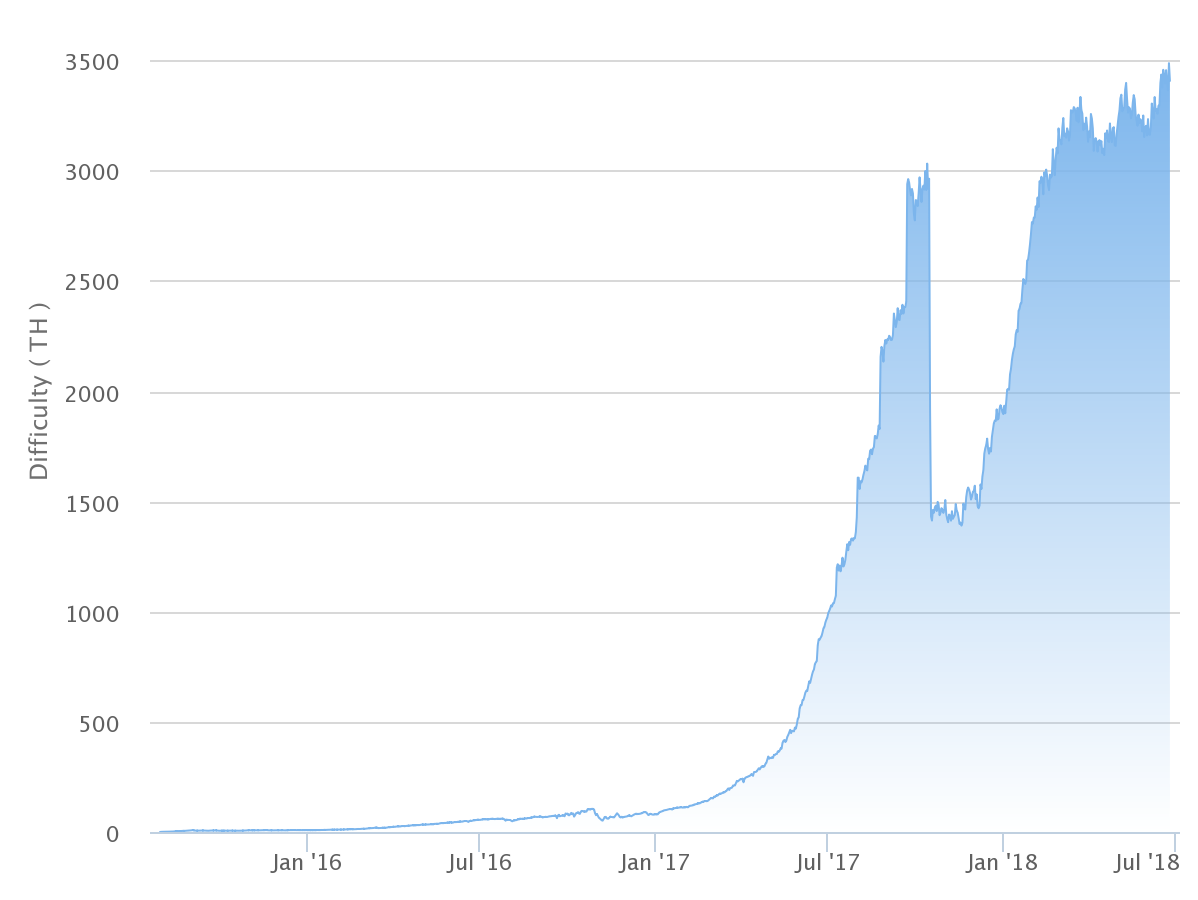
\includegraphics[width=15cm]{imagens/chart.png}
        \caption{Histórico de dificuldade na verificação de blocos no Ethereum \cite{team2017etherscan}.}
        \label{fig:historico-dificuldade-ethereum}
    \end{figure}
    
    Na Figura \ref{fig:historico-dificuldade-ethereum}, nota-se uma queda drástica na dificuldade para minerar novos blocos no Ethereum. Isto ocorreu em Outubro de 2017 devido a um problema na definição do Ethereum que causava uma \textit{bomba de dificuldade}. A Figura \ref{fig:historico-blocktime-ethereum} ajuda a visualizar que, no mesmo período onde houve a redução da dificuldade da geração de blocos, houve também a redução no tempo médio de mineração de blocos.
    
    \begin{figure}[h!]
        \centering
        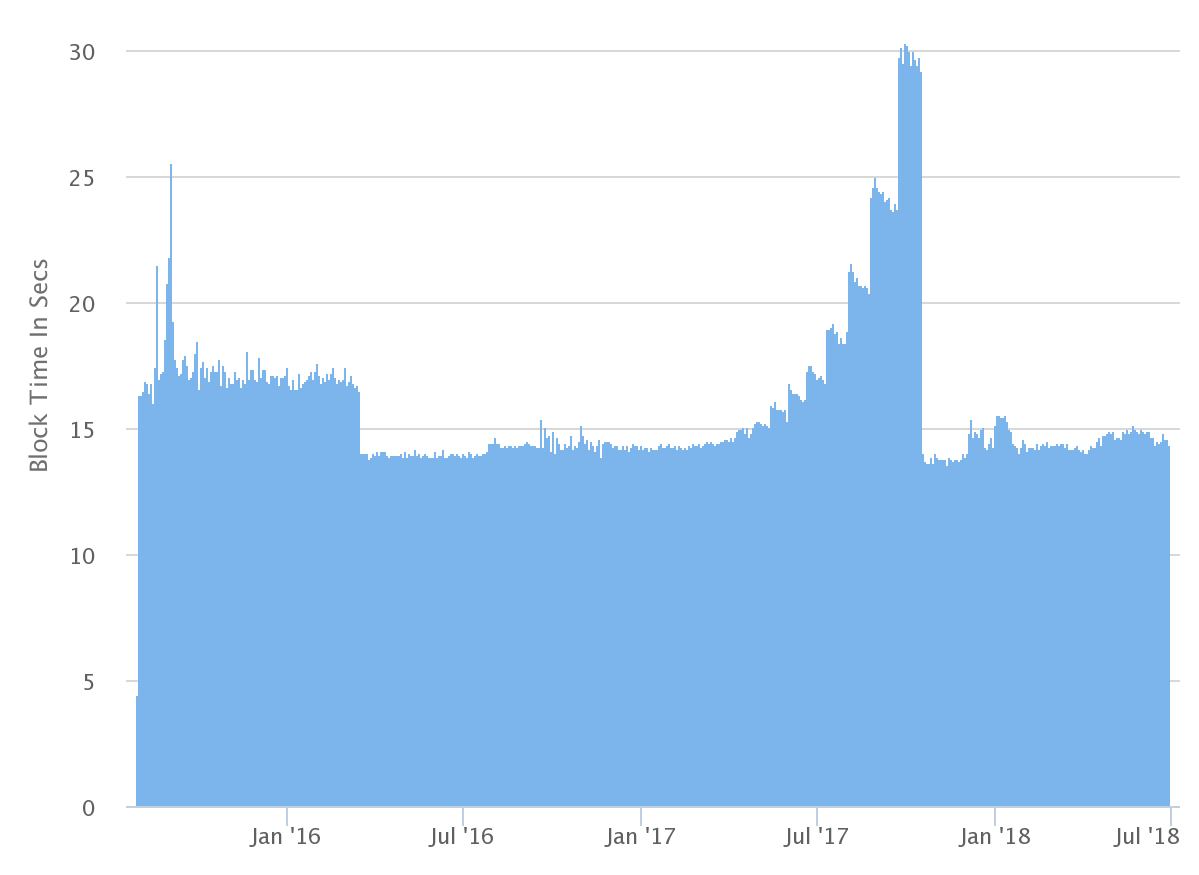
\includegraphics[width=15cm]{imagens/blocktime.png}
        \caption{Histórico de tempo médio gasto para gerar um bloco novo \cite{team2017etherscan}.}
        \label{fig:historico-blocktime-ethereum}
    \end{figure}
    
	Nota-se na Figura \ref{fig:historico-blocktime-ethereum} que, mesmo com o aumento constante da dificuldade em minerar novos blocos, o tempo médio para gerar um novo bloco mantém-se constante.
	
	[conectar as duas partes]
	
	A centralização da informação é, além de um mecanismo de otimização de recursos, uma forma arquitetural no desenvolvimento de sistemas. Sistemas centralizados são fáceis e baratos de serem desenvolvidos, porém sofrem de um problema crítico: possuem uma unidade central que não pode falhar. Uma falha catastrófica do sistema inviabiliza o seu uso, entretanto ataques maliciosos como ataques de negação de serviço podem comprometer o sistema sem que haja uma falha no sistema.
	
    Sistemas decentralizados não possuem um único ponto de falha, uma vez que a informação é distribuída ao longo da rede, tornando-os resilientes a falhas e ataques maliciosos por natureza. Uma arquitetura decentralizada completa deve conter três unidades básicas para o seu funcionamento: unidade de processamento, unidade de armazenamento e uma unidade de troca de mensagens. A rede Ethereum provê as três características necessárias, entretanto um estudo aprofundado sobre a viabilidade e formas de otimização é necessário, uma vez que a computação, no Ethereum, exige um preço. Na proposta deste trabalho, o estudo concentra-se em usar o Ethereum como unidade de processamento e o IPFS como unidade de armazenamento.
    
    A arquitetura da \bchain tem inicio pelo bloco primordial, chamado de \textit{genesis}. Os demais blocos que compõem uma \bchain consistem basicamente de duas partes: dados de transações e valor de hash. Dados de transações consistem em informações que os participantes inserem na \bchain e o valor de hash é uma referência ao bloco diretamente anterior ao bloco atual, é um dado gerado durante o processo de mineração.
	
	[falar como o ethereum pode ajudar neste caso]
	
	[falar sobre iot]
	
	[falar sobre fog computing, iot e porque usar o ethereum nessa área]
	
	Este trabalho utiliza exclusivamente as capacidades do Ethereum em servir como plataforma de desenvolvimento. Embora que o Ethereum tenha um valor econômico e seja utilizado como moeda de troca, este trabalho não visa qualquer estudo nesta área. 
	
	--------------------
	
	Ethereum é uma plataforma que tem como base uma \bchain onde pessoas podem escrever programas, compilar, embarcar os  programas em transações e envia-los como parte de uma transação.
	
	Ethereum 
	
	
	--------------------

\section{Organização da Monografia}
    
    Nesta monografia são utilizados vários termos em inglês; a opção por manter os nomes originais vem da premissa de que esta área de pesquisa é recente e existem muitos estudos na língua inglesa. Manter palavras chave em inglês proporciona maior integração entre trabalhos de diferentes autores, facilitando a integração de conceitos.
    
    A sessão \ref{ssc:trabalhos-relacionados} contém uma seleção de trabalhos importantes relacionados com a arquitetura em \bchain, Ethereum, \textit{Fog Computing}, Internet das Coisas e sistemas decentralizados. A revisão técnica das ferramentas utilizadas neste trabalho é feita no Capítulo \ref{chap:revisao-tecnica}, que contém uma descrição técnica do Ethereum como unidade de computação e IPFS como unidade de armazenamento.
    
    Este trabalho inclui alguns anexos úteis para o melhor entendimento da plataforma Ethereum. O Anexo \ref{annx:taxas-por-instrução} contém uma relação com as taxas em Gas para a execução de programas no Ethereum, já o Anexo \ref{annx:arvore-merkle-patricia} contém uma descrição quanto sobre a árvore Merkle Patrícia, que é a estrutura de dados fundamental para a execução do Ethereum.


%=====================================================%

\chapter{Trabalhos Relacionados}\label{ssc:trabalhos-relacionados}

A pesquisa e o desenvolvimento de sistemas baseados em \bchain é um assunto quente atualmente. Várias frentes buscam a utilização desta tecnologia para a disponibilização de serviços seguros quanto a autenticidade da informação.

Além do Ethereum existem outras plataformas cujo o objetivo é fornecer uma arquitetura em \bchain segura. A busca para o processamento mais eficiente de transações levou no desenvolvimento do EOS, um sistema operacional construído sob uma arquitetura em \bchain. [COMO CITAR ISSO? https://github.com/EOSIO/Documentation/blob/master/TechnicalWhitePaper.md] O EOS é uma plataforma aberta e gratuita para o uso e desenvolvimento de aplicações, e \textit{forks} são naturais e base para o algoritmo de consenso, baseado em Prova de Participação. O grande diferencial para as primeiras versões do EOS, disponibilizadas em junho de 2018 e a versão equivalente do Ethereum no mesmo período, é a velocidade em que transações são processadas na rede principal.

Embora existam poucos recursos confiáveis sobre o funcionamento do EOS, isto é, a principal fonte de informação técnica se resguarda de erros no processo de escrita do documento que descreve a plataforma EOS; é uma plataforma em crescente ascensão que promete ser uma alternativa viável ao Ethereum em poucos anos.

A arquitetura em \bchain é utilizada em várias frentes, como no suporte para o desenvolvimento de nações ou como suporte a um sistema financeiro virtual, \cite{gomez2017creating} lista uma variedade de plataformas em \bchain e aplicações em seu trabalho. Nesta sessão serão apresentados casos de uso de \bchain em geral ou Ethereum.

--- talvez remover ou reescrever esse parágrafo ---

Sistemas de identificação sofrem com o problema da duplicação de dados. No Brasil existem diferentes formas de identificação para uma mesma pessoa: Registro Geral, Cadastro de Pessoa Física, Título Eleitoral, Carteira Nacional de Habilitação, entre outros. Com o Título Eleitoral uma pessoa identificada por seu Registro Geral pode exercer a democracia ao votar no seu candidato durante um período eleitoral. A necessidade de documentos diferentes é reflexo da duplicação de informação.

Governos tecnológicos como a Estônia adotam um sistema de identificação digital. Cada cidadão estoniano possui um único cartão de identificação, utilizado em todos os serviços governamentais. A tecnologia por trás deste sistema é a \bchain KSI (como citar o site?), que promove interoperabilidade entre quase todos os serviços do governo.

--------------

O aumento no uso e desenvolvimento de dispositivos IoT, em que muitas vezes fazem parte de uma rede, requer um sistema flexível o suficiente para permitir o escalonamento sem que haja perdas no nível de segurança. Arquiteturas baseadas em \bchain podem ser 


    A Slock.it busca automatizar processos e interligar nós via \bchain [https://blog.slock.it/slock-it-iot-layer-f305601df963]

[ethembedded , ethereum light client]


    [Falar sobre o EOS que pretende ser concorrente do ethereum?]

    \textbf{falar sobre outras moedas virtuais que possuem a capacidade do ethereum, como o IOTA ou sobre trabalhos cientificos que usam blockchain?}

    
    -=-=-=-=-=-=-=-=-=-=-=-=-=-=-=-=-=-=-=-=-=-=-=-=-=-=-=-=-=-=-=-=
    
    Segundo \cite{spurjeonsurvey}, o Ethereum é a segunda geração das plataformas baseadas em \bchain. Plataformas baseadas em \bchain de segunda geração são mais capazes que o Bitcoin, cuja classificação é a de primeira geração. 
    
    A terceira geração de plataformas baseadas em \bchain estão nascendo neste exato momento e trazem soluções para os problemas de escalabilidade enfrentados pelo Ethereum na sua versão atual, sem considerar as novas propostas que serão discutidas ao longo deste texto. Plataformas de terceira geração abandonam a questão da não existência de governança na \bchain, ou seja, em plataformas de primeira e segunda geração, não existe a crença em participantes especiais que serão para sempre leais ao sistema. Plataformas de primeira e segunda geração garantem a característica de não governança, promovendo um sistema que habilita os próprios participantes formarem organizações com base em regras. No caso do Ethereum, as regras são codificadas em \textit{smart contracts}.
    
    Plataformas de terceira geração habilitam que haja governança na \bchain, onde existem participantes especiais que representam líderes do sistema. Esses tipos de plataforma também promovem a interoperabilidade entre diferentes plataformas. Exemplos de plataformas em \bchain de terceira geração são o Cardano e o IOTA \cite{spurjeonsurvey}.
    
    A maior inovação do Cardano está em seu \textit{design}. A tecnologia por trás do Cardano promove que milhares de transações por segundo sejam realizadas com segurança, isto acontece por conta de duas características:
    
    Cardano é uma ótima tecnologia para operar entre diferentes blockchains, pode suprir as deficiências atuais do Ethereum quanto a escalabilidade, delegando tarefas a outros sistemas de blockchain. Contudo iniciativas como o Ethereum Plasma incentivam que o desenvolvimento deste trabalho seja somente sobre a plataforma Ethereum.
    
    IOTA é um sistema distribuído com foco em Internet das Coisas. O IOTA não é baseado em \bchain, a tecnologia por trás do sistema é chamada de \textit{Tangle} e é definida sob uma estrutura de Grafo Direcional Acíclico (DAG). A tecnologia utilizada no Tangle permite a inexistência de mineradores, logo o funcionamento da plataforma é diferente das tecnologias equivalentes baseadas em \bchain.
    
    Como não existem mineradores no IOTA, cada participante na rede deve participar ativamente no processo de consenso para que possa efetuar transações. Participar ativamente no processo de consenso significa provar pelo menos que duas transações anteriores existem e são válidas, antes que o participante possa realizar a sua transação.
    
    As principais características do IOTA estão na capacidade de escalabilidade do sistema, uma vez que não existem mineradores e o trabalho de validação é distribuído em todos os participantes habilitando o processamento em paralelo de transações. A característica de não possuir mineradores garante que transações sejam processadas sem taxas; o ativo digital relacionado ao IOTA é gerado uma única vez, durante a primeira transação, ou seja, novos \textit{tokens} - ativo digital referente ao IOTA, não são gerados, desta forma a plataforma nunca sofrerá com inflação econômica.
    
    Outra característica do IOTA é a sua função hash, o Curl-P. Segundo a equipe do IOTA, o Curl-P é um algoritmo de geração de hashes que possui imunidade quântica. Entretanto, o algoritmo Curl, versão anterior ao Curl-P, já foi demonstrado que possui falhas criptográficas, permitindo que transações sejam adulteradas \cite{heilman} e a equipe do IOTA encoraja que uma assinatura não seja usada mais que uma vez, devido a natureza da função hash \cite{teamiota}.
    
    O IOTA é uma plataforma que trouxe diferentes visões arquiteturais sobre sistemas decentralizados que possuem um ativo digital envolvido e que permitem o desenvolvimento de aplicações decentralizadas. A principal característica do IOTA é a simplicidade do protocolo, que promove o uso em dispositivos de baixo consumo de energia
    

\chapter{Revisão Técnica}\label{chap:revisao-tecnica}

	%-----------------------------------------------------------------------------------------------------%

\section{Ethereum}\label{ssc:ethereum}

    Ethereum é uma plataforma genérica de computação onde todas as transações são baseadas em conceitos de máquinas de estado e é implementado sobre a arquitetura de \textit{blockchain} \cite{wood2014ethereum}. A ideia do Ethereum é juntar conceitos de execução de código, monetização virtual e protocolos que executam na \textit{blockchain} para permitir o desenvolvimento de aplicações que demandam consenso arbitrário, escalabilidade, padronização e características de completude. Ethereum cumpre os requisitos ao adotar uma arquitetura baseada em \textit{blockchain} com uma linguagem de programação Turing-completa embarcada \cite{buterin2014next}.
    
    O Ethereum além de plataforma para desenvolvimento de aplicações decentralizadas, é uma forma de armazenamento de recursos monetários. O \textit{ether}, moeda virtual da rede principal do Ethereum possui um valor altamente volátil, assim como o valor econômico de qualquer moeda virtual. A aplicação econômica do Ethereum, bem como qualquer tipo de moeda virtual é passível de uma longa discussão econômica, contudo, o âmbito deste trabalho é a exploração das capacidades de desenvolvimento sob a plataforma computacional decentralizada do Ethereum, logo questões econômicas referentes ao Ethereum serão abordadas somente superficialmente ao longo do texto.
    
    O uso do Ethereum como plataforma de computação decentralizada abre um leque de possibilidades único. É possível que \textit{tokens} (no sentido cripto-econômico\footnote{Cripto-economia é o estudo de protocolos que governam a produção, distribuíção e consumo de bens e serviços em uma economia digital e decentralizada. Fonte \textit{https://blockgeeks.com/guides/what-is-cryptoeconomics/}}) sejam desenvolvidos sob o Ethereum, contendo seu próprio valor e sua própria aplicação. 
    
    O Ethereum funciona de acordo com uma máquina de estados baseada em transações definida sob uma arquitetura de \bchain. A partir de um estado inicial, computações são realizadas em sequência e o resultado culmina em um estado final de aceitação ou rejeição. A má formatação do conjunto de instruções que servem de entrada a máquina de estados causa uma parada e o estado atual é revertido ao estado inicial.
    
    Computações no Ethereum são um acrônimo a transações. Uma transação é definida por uma sequência de instruções bem definidas que cumprem um proposito, ou seja, uma transação é um programa executável. Formalmente um programa é conhecido como um contrato inteligente, ou então \textit{smart contract}, que não condiz com o nome e possui inteligência computacional alguma. 
    
    Um \textit{smart contract} pode representar o mesmo que um contrato comum, pode ser definido por uma sequência de clausulas que podem ser aceitas ou não por um participante. Embora os participantes possuam anonimidade na rede, é possível provar qual endereço executou um determinado contrato. Endereços e \textit{smart contracts} são itens públicos no Ethereum e podem ser explorados através de diversas ferramentas, por exemplo, Etherscan \cite{team2017etherscan}.
    
    A especificação do Ethereum não provê uma implementação oficial. Os autores promovem um protocolo bem definido e implementações em diversas tecnologias são encorajadas pela comunidade. Nós Ethereum comunicam-se independente da forma como foram implementados, pois cada nó diferente segue a mesma especificação. Atualmente existem diversas implementações, o site oficial lista três versões principais:
    
    \begin{itemize}
        \item \textbf{Geth}: Implementação completa da especificação do Ethereum em Go, indicado para desenvolvimento Web.
        \item \textbf{Eth}: Implementação do Ethereum em C++, indicado para mineração em placas de vídeo
        \item \textbf{Pyethapp}: Implementação em Python para fins educacionais.
    \end{itemize}
    
    Existem outras implementações do Ethereum, como o Parity, implementado em Rust que é em média 89,8\% mais rápido que o Geth \cite{rouhaniperformance}. O Ethereum funciona em conjunto independente dos clientes, formando uma grande rede, virtualmente um computador global capaz de executar instruções imparáveis.
    
	%-----------------------------------------------------------------------------------------------------%
    
	\subsection{Contas de Participantes}\label{ssc:contas-de-participantes}
	
	Existem dois tipos de contas endereçáveis no Ethereum: contas de usuário externas - EUA e contas de contratos. Contas de contrato são contas onde existe código executável associado, uma execução em um contrato acontece quando uma conta externa envia uma requisição de transação a uma conta de contrato. Os dois tipos de conta no Ethereum contém as seguintes informações:
	
	\begin{itemize}
	    \item \textbf{NONCE}: Valor escalar que representa a quantidade de transações enviadas pela conta, ou a quantidade de contratos criados, caso for uma conta com código associado.
	    \item \textbf{BALANCE}: Valor escalar que representa a quantidade de Wei associada a esta conta.
	    \item \textbf{STORAGE\_ROOT}: Hash de 256 bits do nó raiz da MPT que armazena o conteúdo da conta. 
	    \item \textbf{CODE\_HASH}: Hash que representa o código EVM executável da conta.
	\end{itemize}
	
	Somente uma EUA pode enviar um contrato a ao Ethereum e, como será discutido em \ref{ssc:transacoes}, existe um custo envolvido na ação de submeter um \textit{smart contract} e este custo é calculado em frações de Ether ou unidades de Wei.
	
	Os participantes da rede principal do Ethereum possuem suas contas públicas, onde é possível verificar as movimentações de Ether, os \textit{smart contracts} são públicos por natureza e podem ter seu código auditado por qualquer usuário.

	%-----------------------------------------------------------------------------------------------------%
	
	\subsection{Estado Global}\label{ssc:estado-global}
	
	A execução do Ethereum inicia com um estado chamado de \textit{genesis}. A mudança de estado ocorre na execução de transações. Dado um conjunto de transações válidas e aceitas, estas são armazenadas permanentemente e o estado evolui. O processo de aceitação e validação de transações ocorre na etapa de mineração, que será abordada posteriormente.

	O estado global do Ethereum é representado por uma árvore, essa forma de representação do estado promove um mecanismo de otimização, onde após a adição de um bloco, apenas uma pequena parte da árvore precisa ser modificada. A diferença entre a representação do estado em um bloco e outro deve ser, geralmente, mínima. Dados que são armazenados em um bloco já adicionado à \bchain jamais podem ser modificados, apenas referencias via \textit{hashes}. O estado global do Ethereum é definido via um tipo de árvore chamado de Merkle Patricia - MPT, este esquema permite que um bloco seja apenas inserido ou deletado, jamais modificado. A definição da árvore Merkle Patricia utilizada no Ethereum é encontrada no Anexo \ref{annx:arvore-merkle-patricia}.
	
	O mecanismo de evolução do estado toma como base um conjunto de transações que, quando aceitas levam a um novo estado. Operações no estado levam na ramificação da MPT. A Figura \ref{fig:estado-global-ethereum} ilustra o mecanismo de evolução de estados. 
	
	\begin{figure}
        \centering
        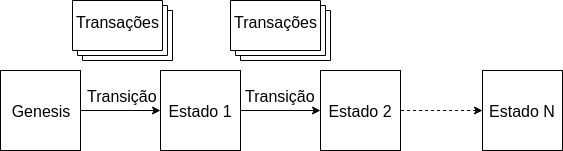
\includegraphics[width=15cm]{imagens/estado-global-ethereum.png}
        \caption{Representação simplificada da execução da máquina de estados do Ethereum.}
        \label{fig:estado-global-ethereum}
    \end{figure}
    
    O leitor pode estar curioso pois a representação do estado global do Ethereum no diagrama se dá em forma de uma lista ligada, entretanto esta é apenas a representação de estados válidos. Operações inválidas ocorrem comumente no Ethereum, seja por má definição de \textit{smart contracts} ou pela ação ilegal de participantes, portanto existem inúmeras ramificações falsas. A arquitetura em \bchain promove os mecanismos suficientes para lidar com esta característica e manter as informações corretas.

	O uso da MPT trás muitos benefícios: a raiz da estrutura de dados é criptograficamente dependente de toda a estrutura de dados interna, portanto, uma assinatura da raiz pode ser seguramente utilizada para garantir a identidade do estado. Todas as raízes do estado global são armazenadas na \bchain e a MPT que define o estado global no Ethereum é uma estrutura de dados imutável, então é possível reverter o estado para qualquer estado anterior, em caso de falha de execução devido a construção incorreta de \textit{smart contracts}.
	
	%-----------------------------------------------------------------------------------------------------%
	
	\subsection{O Bloco}
	
	O bloco é componente primordial em sistemas baseados em \bchain, no contexto do Ethereum, um bloco consiste em um cabeçalho e uma sequência de transações. Em um sistema decentralizado, é necessário combinar um sistema de transições com um sistema de consenso para garantir que todos os participantes concordam com as transações realizadas.
	
	Embora a \bchain do Ethereum seja muito semelhante a \bchain do Bitcoin, existem algumas diferenças. A principal diferença é que cada bloco que compõe a \bchain do Ethereum possui uma cópia da lista de transações e uma cópia do estado mais recente do sistema.
	
	Um bloco é composto por um cabeçalho e uma lista de transações, no qual o bloco possui a seguinte estrutura:
	
	\begin{itemize}
	    \item \textbf{PARENT\_HASH}: A hash KEC do cabeçalho do bloco pai.
	    \item \textbf{OMMERS\_HASH}: A hash KEC da lista de blocos \textit{ommer}.
	    \item \textbf{BENEFECIARY}: Um endereço de 160 bits para onde as taxas de mineração serão depositadas.
	    \item \textbf{STATE\_ROOT}: A hash KEC do nó raíz da arvore de estados após todas as transações serem processadas e finalmente aplicadas.
	    \item \textbf{TRANSATIONS\_ROOT}: Hash para a raíz da MPT de transações referentes ao bloco.
	    \item \textbf{RECEIPTS\_ROOT}: Hash para a raiz da trie dos endereços que recebem fundos em cada transação.
	    \item \textbf{LOGS\_BLOOM}: Registro de eventos referentes ao bloco.
	    \item \textbf{DIFFICULTY}: Um valor inteiro que indica a dificuldade para minerar o bloco.
	    \item \textbf{NUMBER}: Valor inteiro que representa o número de blocos antecessores.
	    \item \textbf{GAS\_LIMIT}: Valor que representa o limite de Gas que pode ser usado para minerar o bloco.
	    \item \textbf{GAS\_USED}: Valor que indica a quantidade de Gas utilizado para minerar o bloco.
	    \item \textbf{TIMESTAMP}: Carimbo de tempo que indica quando o bloco foi criado.
	    \item \textbf{EXTRA\_DATA}: Um arranjo de bytes de dados arbitrários com tamanho máximo de 32 bytes.
	    \item \textbf{MIX\_HASH}: Uma hash de 256 bits que, junto do NONCE, prova que foi utilizado uma quantidade suficiente de trabalho na mineração do bloco.
	    \item \textbf{NONCE}: Uma hash de 64 bits que, junto do MIX\_HASH, prova que foi utilizado uma quantidade suficiente de trabalho na mineração do bloco.
	\end{itemize}
	
	Cada bloco é ligado a seu antecessor através do \textbf{PARENT\_HASH}. Esta é forma primordial de segurança contra a adulteração de dados na \bchain, onde a modificação em qualquer byte do bloco anterior quebra a cadeia de blocos e a \bchain torna-se inválida para o participante que está tentando modificar informações já registradas.
	
	Blocos são gerados constantemente através do processo de mineração, onde participantes mineradores usam seu poder computacional para validar todas as transações contidas no bloco. Em troca, o primeiro minerador a terminar o processo de verificação, recebe taxas referente ao procedimento executado. É no momento da mineração de blocos que novas cifras de \textit{ether} são geradas e a cada bloco minerado, a complexidade para minerar o próximo bloco aumenta como forma de controlar a inflação do \textit{ether}.
	
	Cada bloco já minerado na rede principal do Ethereum é aberto e livre para ser inspecionado. A ferramenta Etherscan \cite{team2017etherscan} permite, além de explorar os blocos que compõe a \bchain do Ethereum, também verificar os sistemas de \textit{tokens} desenvolvidos com base no Ethereum.
	
	A validação de blocos ocorre através de uma prova matemática, chamado de prova de trabalho - PoW. Cada sistema baseado em \bchain implementa seu próprio algoritmo de PoW, no caso do Ethereum o algoritmo que realiza a verificação dos blocos no modelo de PoW é chamado de \textit{Ethash}. Esta informação é importante pois o Ethereum está passando a realizar a verificação de blocos via prova de participação - PoS, onde a participação de mineradores será irrelevante.
	
	Enquanto não há a transição do modelo de PoW para PoS, o Ethereum mantém o tempo médio para a mineração de um bloco em torno de 12 segundos, o que é um péssimo tempo de resposta ao comparar o sistema de computação do Ethereum com serviços de nuvem centralizados.


	%-----------------------------------------------------------------------------------------------------%
    
	\subsection{Transações}\label{ssc:transacoes}
	
	Em Ethereum, uma transação é uma troca de mensagem entre duas contas que alteram o estado do Ethereum. Dois tipos de transações podem ocorrer: transações cujo endereço de destino é uma EUA, o valor da transação é transferido a conta destino; em transações cujo endereço de destino é um endereço de um contrato, o dado armazenado no campo \textbf{DATA} é usado como parâmetro para a execução do contrato. Uma transação é um objeto cujos campos são:
	
	\begin{itemize}
	    \item \textbf{NONCE}: Valor que representa o número de transações enviadas pela conta que invocou a transação.
	    \item \textbf{GAS\_PRICE}: Valor que representa a quantidade de Wei a ser paga por unidade de Gas utilizada no processamento da transação.
	    \item \textbf{GAS\_LIMIT}: Valor que representa a quantidade máxima de Gas que pode ser utilizada no processamento da transação.
	    \item \textbf{TO}: Endereço destino da transação caso não seja uma operação de criação de contrato, caso contrário, este campo é vazio.
	    \item \textbf{VALUE}: Valor que representa a quantidade de Wei a ser transferida na transação.
	    \item \textbf{V, R, S}: Valores correspondentes a assinatura da transação; são utilizados para determinar o endereço que invocou a transação.
	    \item \textbf{INIT}: Arranjo de bytes que representa o código EVM no procedimento de criação de contrato.
	    \item \textbf{DATA}: Arranjo de bytes que representa o dado de entrada na invocação do contrato.
	\end{itemize}
	
	Quando uma EUA executa uma transação, esta é assinada com a chave privada da conta que deu origem a transação e então esta transação é direcionada aos nós do Ethereum mais próximos (o que pode ser um nó executando localmente), e estes nós se encarregam de propagar a transação ao restante da rede; se um nó minerador aceitar a transação, então a transação é incluída no processo de mineração. A transação somente é executada no processo de mineração, onde ocorre a mutação do estado.
	
	Transações podem ser ignoradas caso o \textbf{GAS\_PRICE} for abaixo do esperado pelo nó, pois é a partir do \textbf{GAS\_PRICE} que as taxas de mineração são pagas ao minerador. Se, durante a execução de uma aplicação é necessário que uma transação seja efetuada cujo \textbf{GAS\_PRICE} envolvido é baixo o suficiente para nenhum minerador aceitar a transação, é possível re-transmitir a transação para a rede com outro valor de \textbf{GAS\_PRICE} com o mesmo valor de \textbf{NONCE} da transação não aceita. Uma vez aceita e minerada, a transação pode ser acessada por qualquer nó na rede enquanto residir no nó em que esta foi aceita.
	
	Uma transação aceita cujo \textbf{GAS\_PRICE} associado é muito baixo, pode eventualmente ser descartada pelo minerador, pois o número de transações armazenadas é finito. Se nenhum nó na rede possui o registro da transação, ela é lançada novamente no sistema para que seja aceita por algum nó. A transação permanecerá no estado de pendente enquanto não for aceita por nenhum nó minerador, é possível acompanhar as transações pendentes na rede principal do Ethereum no através do Etherscan \cite{team2017etherscan}.

	%-----------------------------------------------------------------------------------------------------%
	
	% \subsection{Ethash}\label{ssc:ethash}
	
	%-----------------------------------------------------------------------------------------------------%
	
	\subsection{\textit{Smart Contracts}}
	
	O conceito de \textit{smart contracts} data da década de 90. Nick Szabo introduziu o conceito de \textit{smart contracts} como um protocolo de transação computadorizado que executa em termos de um contrato, na qual as cláusulas contratuais são traduzidas em código executável em algum meio digital \cite{szabo1997}.
	
	Ethereum é uma plataforma com suporte a aplicações com cunho financeiro e aplicações que possuem nenhuma aplicação econômica. Este tipo de característica é altamente associada ao conceito de contratos inteligentes - \textit{smart contracts}. Um \textit{smart contract} é um programa escrito em alguma linguagem que, após compilado e gerado um código executável, é então executado em uma camada da \textit{blockchain} do Ethereum.
	
	Qualquer usuário pode escrever e enviar um \textit{smart contract} para a \textit{blockchain}. Um contrato após deposto na \textit{blockchain} pode interagir com outros contratos por meio de trocas de mensagens, assim como usuários também podem interagir com contratos, depositando ou enviando fundos de uma conta a outra por meio de transações.
	
	Existem diversas linguagens de programação de alto nível de abstração que são compiladas para o código EVM. Neste trabalho é utilizado a linguagem de programação Solidity \cite{dannen2017introducing} para a implementação dos \textit{smart contracts} que compõem a prova de conceito.

	%-----------------------------------------------------------------------------------------------------%

	\subsection{Gas}
	
	Gas é uma unidade de consumo de processamento, usado para evitar abusos da rede e para garantir a completude dos \textit{smart contracts}, ou seja, todos os contratos da rede Ethereum são sujeitos a taxas. Estas taxas são calculadas a partir da execução do código dos contratos pelos mineradores. Cada transação em Ethereum exige uma quantidade limite de Gas que pode ser consumida, conhecido como \textbf{GASLIMIT} e a quantidade de Gas dispendida a cada etapa da execução é calculada utilizando como parâmetro o \textbf{GASPRICE}. O conceito de Gas em Ethereum é equivalente a quantidade de combustível presente em um veículo. Para um veículo percorrer a distância da origem \textit{A} ao destino \textit{B}, é necessário uma certa quantidade de combustível, se o combustível acabar durante o trajeto, o veículo fica parado em algum ponto entre \textit{A} e  \textit{B}. Equivalente no Ethereum, se a execução de um contrato necessitar de uma quantidade maior de Gas que a origem da transação está disposta a pagar, a execução é interrompida e a transação descartada.
	
	A origem na qual deseja invocar uma transação pode especificar o preço da computação, isto é, o \textbf{GASPRICE}, assim como os mineiros podem ignorar as transações, se assim desejarem. Um valor maior de \textbf{GASPRICE} aumenta o interesse dos mineiros em executar o contrato requisitado ao passo que torna a transação mais cara para a conta de origem. As taxas restantes ta mineração que não são devolvidas a origem ou movidas a uma conta de destino, são depositadas no endereço \textbf{BENEFICIARY}.

	%-----------------------------------------------------------------------------------------------------%
    
	\subsection{Ethereum Virtual Machine}
	
	A Ethereum Virtual Machine - EVM, é um mecanismo que implementa um modelo de execução que permite a manipulação do estado com base em uma sequência de instruções e uma representação de ambiente baseada em tupla. A EVM é uma máquina de estados virtual \textit{quasi}-Turing completa, pois a quantidade de instruções executada é limitada por um valor superior chamado \textbf{GASLIMIT} - introduzido anteriormente.
	
	A arquitetura da EVM é baseada em uma máquina de pilha, cujo tamanho da palavra é de 256 bits, o que facilita o uso em conjunto com o KEC. O modelo de memória da EVM possui dois componentes: a pilha de execução cujo tamanho máximo é de 1024 instruções e um espaço de armazenamento não volátil que é mantido como parte do estado do sistema. Ambos componentes de memória são inicializados com o valor zero.
	
	O mecanismo de escrita do código executável na memória da EVM é particular. Através de uma função especial, encapsulada por um limite de Gas que pode ser utilizado para enviar um \textit{smart contract} a blockchain, um código executável é escrito em uma memória de somente leitura. Ou seja, um \textit{smart contract} quando deposto na blockchain torna-se uma lista de instruções imutáveis.
	
	As execuções de \textit{smart contracts} são encapsuladas por uma região segura para execução de instruções, garantindo que os fundos gastos para a execução malsucedida de um contrato sejam devolvidos a conta que invocou a execução. Exceções ocorrem por diversos motivos, como o consumo máximo de Gas ser atingido ou a execução inválida de instruções.
	
	As taxas de execução são cobradas em três circunstâncias: na execução das instruções de um contrato, no envio ou execução de um contrato e no uso de memória pela EVM. Este trabalho contém uma listagem com a taxa para a execução de instruções e se encontra no Anexo \ref{annx:taxas-por-instrução}.
  
	%-----------------------------------------------------------------------------------------------------%
    
    \subsection{Protocolo Casper}
    
    Um dos maiores objetivos de sistemas em \textit{blockchain} é a habilidade de não permitir que transações sejam desfeitas, como uma movimentação de valores econômicos de uma conta a outra ou a execução de um contrato inteligente, no caso do Ethereum. A rede principal do Ethereum é responsável por esta característica, onde blocos de transações aceitas nunca poderão ser copiados e então aceitos novamente.
    
    Este tipo de falha está associada ao clássico problema dos generais bizantinos, onde uma falha de comunicação intencional ou não compromete o consenso do grupo de generais que acreditam na lealdade de todos componentes do grupo. Um general traidor pode transmitir duas mensagens diferentes para dois grupos diferentes de generais, causando um acordo falho. O problema dos generais bizantinos é um problema clássico de sistemas de computação distribuída.
    
    Existem inúmeros algoritmos que lidam com o problema dos generais bizantinos \cite{coulouris}, o protocolo Casper segue os algoritmos clássicos que tratam de falhas bizantinas baseando-se em sistemas PoS.
    
    Em um sistema PoS, novos blocos são aceitos e adicionados a \textit{blockchain} por um processo onde qualquer participante que possua moedas aceitas no sistema pode participar. A influência de um participante é equivalente ao número de moedas que este participante possui, ou seja, quanto maior a quantidade de moedas, maior sua influência sobre o sistema PoS. Esta abordagem é muito mais eficiente que a alternativa PoW, onde novos blocos são aceitos e adicionados a \textit{blockchain} somente através do processo de mineração \cite{buterin2017}. Um sistema PoS pode operar sem um hardware dedicado para mineração, barateando os custos para manter o sistema.
    
    Em uma primeira versão, o protocolo Casper será um sistema hibrido de PoS/PoW, isto é, um sistema PoS executando em camada sobre o atual algoritmo de PoW do Ethereum, no qual adiciona as seguintes características ao Ethereum:
    
    \begin{itemize}
        \item \textbf{Prestação de contas}: Se um validador do sistema violar alguma regra, é possível identificar o validador e a regra violada. A penalização é dinâmica e varia de acordo com o tamanho da violação do sistema por um validador traidor, causando perdas de moedas. Este mecanismo provoca maiores incentivos para que os participantes não violem regras, garantindo a segurança do sistema.
        \item \textbf{Validadores dinâmicos}: É possível que os validadores mudem ao longo do tempo, sem comprometer o sistema.
        \item \textbf{Defesa}: Se mais de 1/3 dos validadores, por algum motivo, ficarem offline, o sistema é capaz de sincronizar com o resto dos validadores e manter o consenso e a segurança.
        \item \textbf{Modular}: O design do protocolo Casper como uma camada torna a implementação facilitada sob uma \textit{blockchain} já existente que executa PoW.
    \end{itemize}
    
    A adição do protocolo Casper ao Ethereum garante a tolerância de dois tipos de falhas: \textit{revisores de longa data} e \textit{falhas catastróficas}.
    
    Em uma falha de revisores de longa data, se um grupo de validadores removem seus fundos do sistema e os fundos deste grupo de validadores contém 2/3 ou mais da quantidade total de fundos, o grupo poderia utilizar de sua superioridade para finalizar situações conflitantes sem que sejam punidos. Uma falha catastrófica ocorre quando uma quantidade maior que 1/3 dos validadores entram em processo de falha ao mesmo tempo.
    
    O protocolo Casper é uma camada que realiza PoS sob a atual camada que realiza PoW no Ethereum, embora adicione características de segurança e velocidade na computação de transações a rede, o protocolo não é perfeito e ainda não é suficiente para prevenir ataques de 51\%. Detalhes técnicos do procolo Casper podem ser encontrados em \cite{buterin2017}.
    
	%-----------------------------------------------------------------------------------------------------%
    
%    \subsection{Ethereum Plasma}

% 	%-----------------------------------------------------------------------------------------------------%
    
%     \subsection{Aplicações}
    
%     [falar sobre aplicações em áreas financeiras]
    
%     [aplicações em organizações decentralizadas]
    
%     [aplicações em iot]
    
\section{Interplanetary File System}

    O \textit{InterPlanetary File System} - IPFS é um sistema de arquivos distribuído \textit{peer-to-peer} (P2P) que busca conectar todos os dispositivos com o mesmo sistema de arquivos \cite{benet2014ipfs}. O IPFS tem este nome por conta da sua definição, o sistema foi desenvolvido com foco em tecnologias futuras de exploração interplanetária, onde a comunicação entre a origem da informação e o ponto requisitante possui latência na ordem de minutos ou horas. O IPFS permite que uma versão de uma informação - uma parte da internet, por exemplo - seja armazenada via IPFS em um local e ser atualizada de tempos em tempos com a versão mais atual via versionamento, ou seja, o IPFS permite a comunicação via internet entre diferentes planetas.
    
    A estrutura de dados que dá suporte ao IPFS é a árvore Merkle.
    
    Vários projetos utilizam o IPFS como base para a construção de uma internet cujo endereçamento é feito com base no conteúdo e não na origem do conteúdo. Um arquivo pode residir em diferentes computadores, mas é acessado através de uma hash que representa este arquivo.
    
    Diferentemente do protocolo HTTP, onde o conteúdo é endereçado baseado na sua localidade e tem como principal ponto de falha o servidor que armazena o conteúdo, o IPFS provê o endereço baseado no conteúdo. Cada arquivo é endereçado por uma hash que representa o arquivo, existe apenas uma hash por arquivo e, se um único bit do arquivo for modificado, a hash que representa este arquivo será diferente. O mecanismo de endereçamento do IPFS permite que o conteúdo acessado através da hash seja verificável, o que garante a consistência de arquivos em redes inseguras.
    
    O armazenamento de arquivos no IPFS é feito com base em arquivos objeto, que são objetos que representam um arquivo. Um objeto-arquivo contém um campo de dados, cujo tamanho máximo é de 256 kilobytes e uma lista de links para outros objetos no IPFS. Arquivos maiores que 256KB são divididos em múltiplas porções e armazenados em diferentes objetos-arquivo. A Figura \ref{fig:arquivo-objeto-ipfs} ilustra este mecanismo.
    
    \begin{figure}[h!]
        \centering
        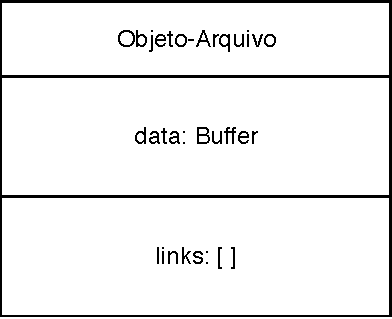
\includegraphics[width=6cm]{imagens/arquivo-objeto-ipfs.pdf}
        \caption{Representação de um arquivo por meio de um objeto no IPFS.}
        \label{fig:arquivo-objeto-ipfs}
    \end{figure}
    
    Arquivos que requerem mais de um objeto-arquivo para armazenar o seu conteúdo, são representados por um objeto-arquivo cujo campo de dados é vazio e o campo de links é populado por todas as hashes de objetos-arquivo que compõe o arquivo maior que 256KB, este mecanismo é representado na Figura \ref{fig:representacao-arquivo-grande-ipfs}.
    
    \begin{figure}[h!]
        \centering
        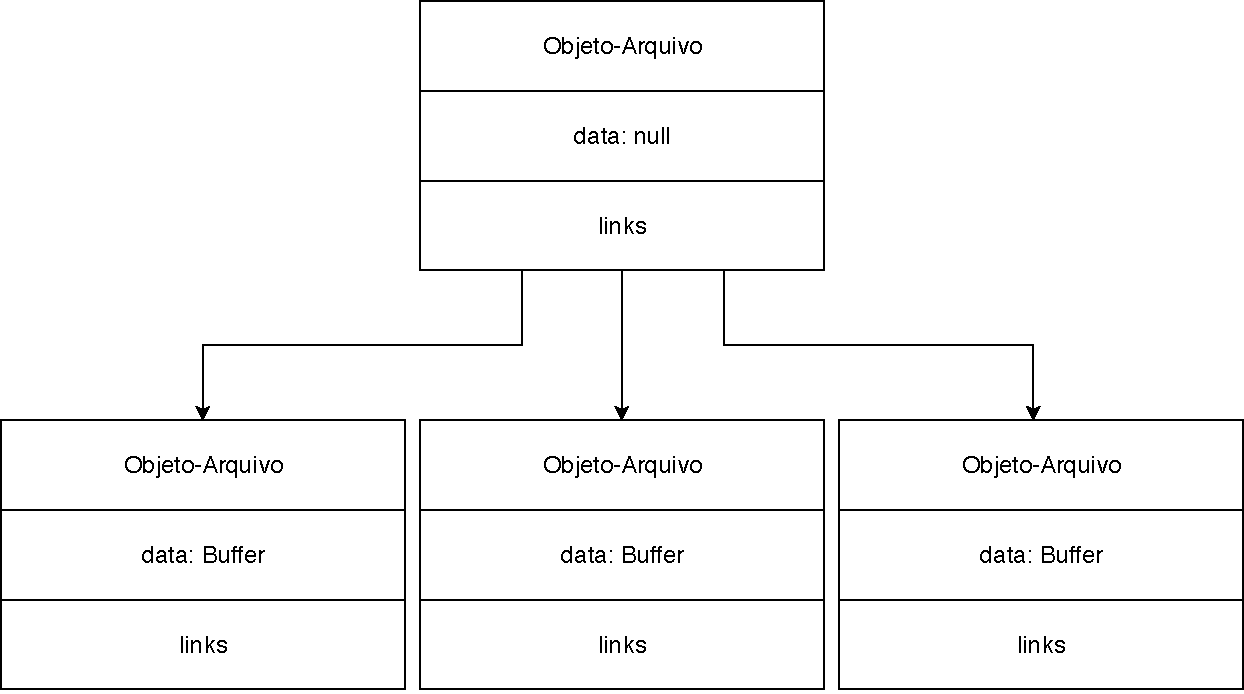
\includegraphics[width=15cm]{imagens/representacao-arquivo-grande-ipfs.pdf}
        \caption{Representação de um arquivo grande por meio de um objeto no IPFS.}
        \label{fig:representacao-arquivo-grande-ipfs}
    \end{figure}
    
    A estrutura de armazenamento de arquivos no IPFS permite que haja armazenamento recursivo, o que dá suporte a diretórios. Esta característica faz com que o IPFS possa ser utilizado como um sistema de arquivos imutável. Ou seja, um arquivo adicionado ao IPFS poderá ser excluído somente se todos os nós que contém uma cópia do arquivo excluam sua versão do arquivo.
    
    O IPFS permite a modificação de arquivos via versionamento, um objeto \textit{Commit} representa uma versão de um objeto-arquivo, toda vez que um arquivo for modificado, é gerado um novo objeto Commit que possui uma referência ao Commit anterior. A Figura \ref{fig:representacao-commit-ipfs} ilustra este mecanismo, que é semelhante ao mecanismo de blockchains.
    
    \begin{figure}[h]
        \centering
        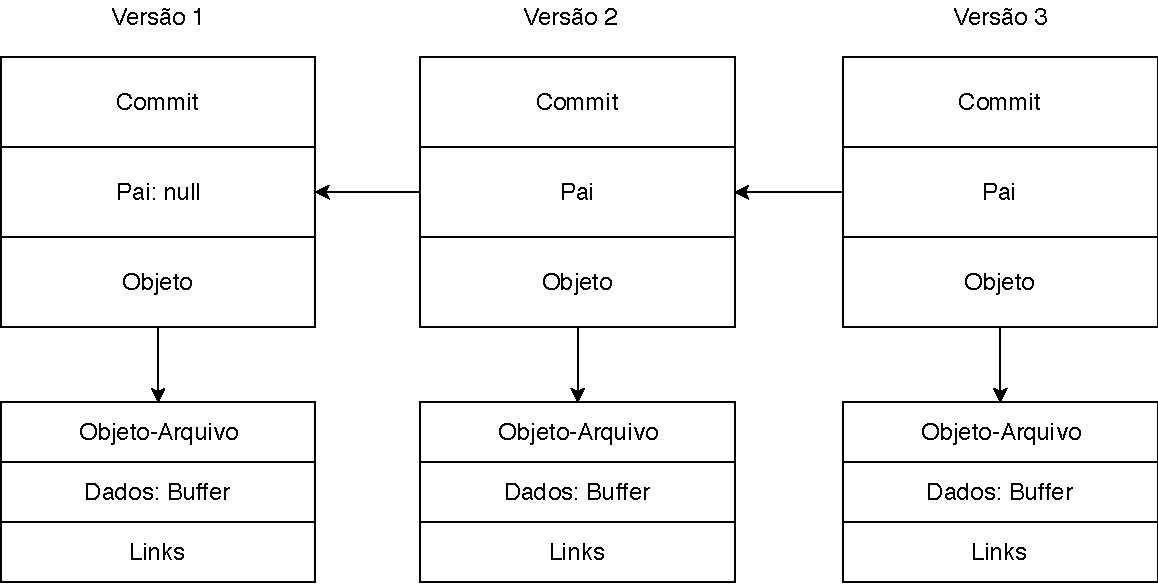
\includegraphics[width=16cm]{imagens/representacao-commit-ipfs.pdf}
        \caption{Representação do versionamento de um objeto-arquivo no IPFS.}
        \label{fig:representacao-commit-ipfs}
    \end{figure}
    
    Existem iniciativas que visam tornar o conhecimento da humanidade não censurável e resiliente de tal forma que nunca seja apagado, este é o caso da Wikipédia. Em 2017 o governo turco decidiu censurar o acesso da população a Wikipédia, este acontecimento motivou a organização Turkey Blocks em conjunto com a equipe do IPFS, a mover uma ação que visava disponibilizar a Wikipédia via IPFS\footnote{https://ipfs.io/blog/24-uncensorable-wikipedia/ - Acessado em Julho de 2018}. Por conta da natureza distribuída do IPFS, ele não pode ser bloqueado simplesmente restringindo o acesso a determinados endereços IP.

	\subsection{Arquitetura}
	    
	    A arquitetura do IPFS sintetiza as principais técnicas de versionamento de distribuição de conteúdo via rede P2P, como a tecnologia do BitTorrent, Git e SFS através de uma DHT. A principal característica deste sistema de arquivos distribuído.
    
    	\subsubsection{Identidade}
        
        \subsubsection{Rede}
        
        \subsubsection{Rotas}
        
        \subsubsection{Trocas}
        
        \subsubsection{Objetos}
        
        \subsubsection{Arquivos}
        
        \subsubsection{Sistema de nomes}
    
    \subsection{Limitações}
    
    Um dos principais problemas do IPFS está na sua natureza. Por ser um sistema de arquivos imutável, qualquer conteúdo adicionado ao IPFS permanecerá no IPFS enquanto houver alguma réplica daquele conteúdo existindo em algum nó participante. Conteúdos digitais protegidos por direitos autorais não podem ser censurados a menos que todos os nós que armazenam uma cópia do arquivo sejam derrubados.
    
    Além da censura de conteúdo, o acesso a arquivos presentes no IPFS ainda é difícil para os usuários em geral por conta da natureza do IPFS. Embora uma página web estática possa ser armazenada completamente no IPFS, o acesso a essa página pelo navegador exige o uso de uma camada de software capaz de interconectar o protocolo do IPFS com o protocolo HTTP. Para tal, existe o serviço de nomes - IPNS que lida com esta tarefa.
    
    O IPFS não executa ações sem que o usuário invoque-as explicitamente. Todo conteúdo deve ser replicado manualmente ou por algum processo automático de replicação. Protocolos desenvolvidos com base no IPFS, como o Filecoin, conseguem efetuar a replicação do conteúdo automaticamente \cite{jbenet47issue}.
    
    Outro problema que o IPFS enfrenta é a disponibilização de conteúdo. Se dois nós armazenam um determinado conteúdo e se, em algum instante de tempo, ambos os nós estiverem desconectados da rede do IPFS, o conteúdo estará indisponível para qualquer usuário que tente acessá-lo. O Filecoin é uma iniciativa para promover que nós armazenem arquivos em troca de uma moeda virtual \cite{protocollabs}, entretanto ainda está disponível apenas em modo ICO - \textit{Initial Coin Offering}.
    
    O IPFS consegue ser um substituto completo do protocolo HTTP, entretanto não há um equivalente ao protocolo HTTPS, ou seja, na versão atual o IPFS não lida com certificados 
        
%=====================================================%

\chapter{Modelagem}

%=====================================================%
%              Fim da monografia parcial              %
%=====================================================%

% \chapter{Desenvolvimento}

%=====================================================%

% \chapter{Resultados}

%=====================================================%

% \chapter{Conclusão}



% Bibliografia http://liinwww.ira.uka.de/bibliography/index.html um
% site que cataloga no formato bibtex a bibliografia em computacao
% \bibliography{nomedoarquivo.bib} (sem extensao)
% \bibliographystyle{formato.bst} (sem extensao)

\bibliography{bibliografia} 
\bibliographystyle{abnt}
%\bibliographystyle{plain}

% Anexos (Opcional)
\annex
\chapter{Tabela de taxas por instrução}\label{annx:taxas-por-instrução}

[listagem das taxas por instrução]

\chapter{Árvore Merkle Patricia}\label{annx:arvore-merkle-patricia}

\section{Versão modificada do Ethereum}

\end{document}

